% !TEX root = catron-dissertation.tex
\epstopdfsetup{outdir=./images/01_introduction/}

\chapter{Introduction}
\label{chap:01_intro}

Directed-energy systems have a variety of uses but typically fall into one of two categories: communications and weapons.
The primary benefits of directed-energy communications is the ability to have secure point-to-point data transfer that is high unlikely to intercept or be interfered with \cite{crs-2021-RwNjGeZD}.
Directed-energy weapons are likely to have a lower cost per shot and a deeper magazine when compared to traditional munitions \cite{crs-2021-hyCUE868}.
As ground based directed-energy systems are slowly rolled out, most prominently aboard the USS Ponce \cite{crs-2021-Atxb7GDv}, there is a desire to field a system aboard an aircraft.

There have been two major attempts to field a directed-energy system aboard an aircraft to date \cite{Jumper-2013-8KtN3pue}.
The first was the Airborne Laser Laboratory (ALL) which took place in the late 1970's and early 1980's which used a CO$_2$ laser at 10.6-$\mu$m.
The second was the Airborne Laser (ABL) program which operated in the 2000's and used a COIL laser at 1.315-$\mu$m.
Airborne optical systems have to deal with a phenomenon know as ``aero-optics,'' which is optical distortions caused by various aero-dynamic flow features.
These optical distortions were first noticed due to image degradation in wind tunnel measurements in the 1950's \cite{Stine-1956-UaRzVZCe} as well as in photo-reconnaissance missions in the 1960's \cite{Kyrazis-2013-vwKeEBym}.

The intensity of that makes through an optical disturbance to a target, $I$, divided by the diffraction-limited performance, $I_0$, is known as the Strehl ratio \cite{Mahajan-1982-kkXM4eaB}, $\sr$,
\begin{equation}
  \sr = \frac{I}{I_0} \textrm{.}
  \label{eqn:01_strehl_ratio_definition}
\end{equation}
The diffraction-limited performance is the intensity that would make it to the same target if not for a disturbance.
The Airborne Laser Laboratory had an estimated Strehl ratio of 95\%\cite{Jumper-2013-8KtN3pue} meaning the ``aero-optics problem'' effectively did not apply.
After the Airborne Laser Laboratory program there was a desire to move toward shorter wavelengths in order to take advantage of improved diffraction-limited performance \cite{Jumper-2001-6QDh7zDy},
\begin{equation}
  \frac{I_0}{P} = \frac{1}{\pi}\left(\frac{Ap}{\lambda z}\right)^2 \textrm{,}
  \label{eqn:01_farfield_intensity}
\end{equation}
where $P$ is the laser output power, $Ap$ is the aperture size, and $z$ is the propagation distance.
This improved diffraction-limited performance is shown in Figure \ref{fig:01_farfield_intensity}.
\begin{figure}
  \centering
  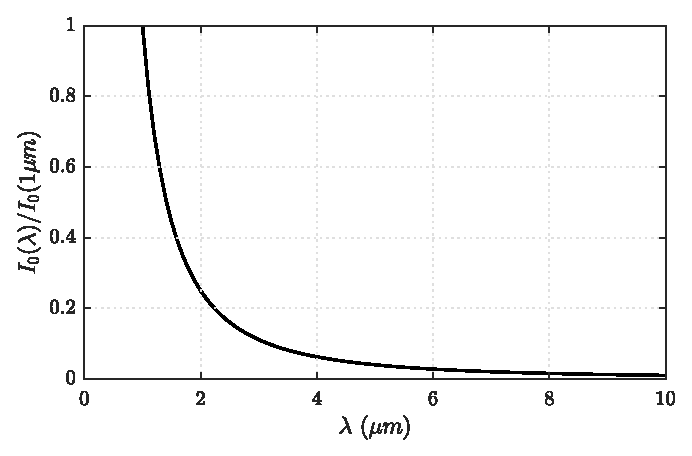
\includegraphics{../matlab/01_introduction/farfield_intensity.eps}
  \caption{Diffraction-limited far-field intensity of a beam normalized by the performance at 1-$\mu$m.}
  \label{fig:01_farfield_intensity}
\end{figure}
By only changing the laser source from a 10-$\mu$m to 1-$\mu$m wavelength the diffraction-limited performance can be increased 100 times.

Aero-optical issues start to become apparent as the wavelength is decreased as is evident by the Mar\'echal approximation \cite{Mahajan-1983-hg7ahvJM} which relates the Strehl ratio to wavelength,
\begin{equation}
  \sr \approx \exp\left\{-\left[\frac{2\pi \opdrms}{\lambda}\right]^2\right\} \textrm{,}
  \label{eqn:01_strehl_ratio}
\end{equation}
where $\opdrms$ is the spatial root-mean-square of the optical path difference over the aperture and will be further discussed later.
If the ALL system's laser was swapped with another laser of a lower wavelength, the Strehl ratio would significantly decrease as shown by Figure \ref{fig:01_strehl_ratio}.
\begin{figure}
  \centering
  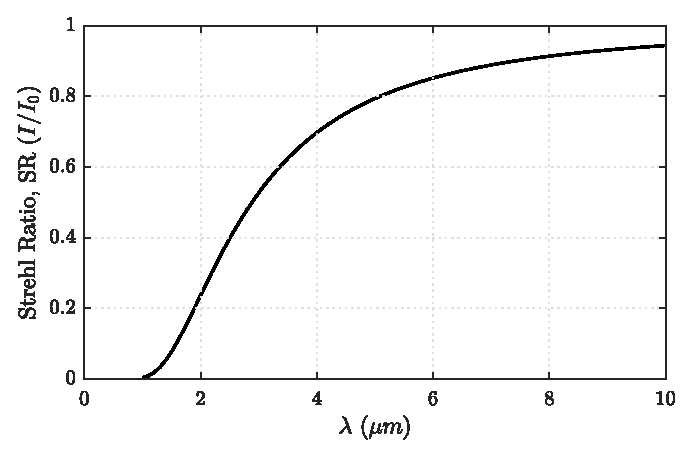
\includegraphics{../matlab/01_introduction/strehl_ratio.eps}
  \caption{Strehl ratio due to the $\opdrms$ of the Airborne Laser Laboratory (ALL) at various laser wavelengths.  ALL had an estimated Strehl ratio of 95\% with its 10.6-$\mu$m laser.}
  \label{fig:01_strehl_ratio}
\end{figure}
While the hypothetical case of going from 10 to 1-$\mu$m resulted in a 100-fold increase in diffraction-limited performance, the actual on-target intensity that this hypothetical system obtains would be essentially zero.
This means that the aero-optical problem can no longer be ignored and was recognized as one of the main developmental risks of the ABL program \cite{DOTE-1999-HnkadUEw}.




% \begin{figure}
%   \centering
%   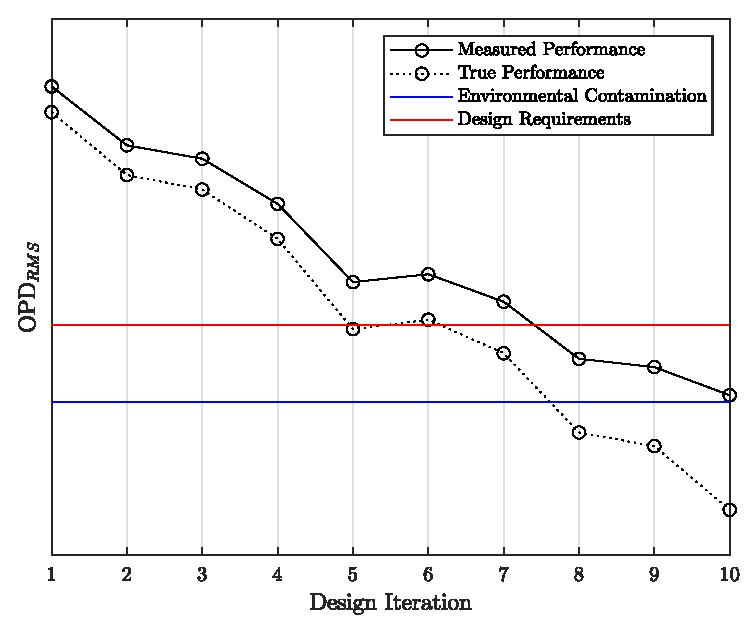
\includegraphics{../matlab/01_introduction/design_iteration.eps}
%   \caption{title}
%   \label{fig:01_design_iteration}
% \end{figure}
%
%
%
% The best possible performance of a directed energy system whether airborne or ground based in the far-field is the diffraction-limited case.
% The far-field intensity of a diffraction-limited beam in represented by $I_0$ and defined in Equation \ref{eqn:01_farfield_intensity},
% \begin{equation}
%   I_0 = \left(\frac{kAp^2}{8z}\right)^2
%   \label{eqn:01_farfield_intensity}
% \end{equation}
% where $k$ is the wavenumber of the beam, $Ap$ is the aperture size, and $z$ is the distance from the aperture to the far-field.
% Figure \ref{fig:01_farfield_intensity} show the far-field diffraction-limited intensity of a beam as the wavelength of the beam is varied and normalized by $I_0$ at 1$\mu$m.
% \begin{figure}
%   \centering
%   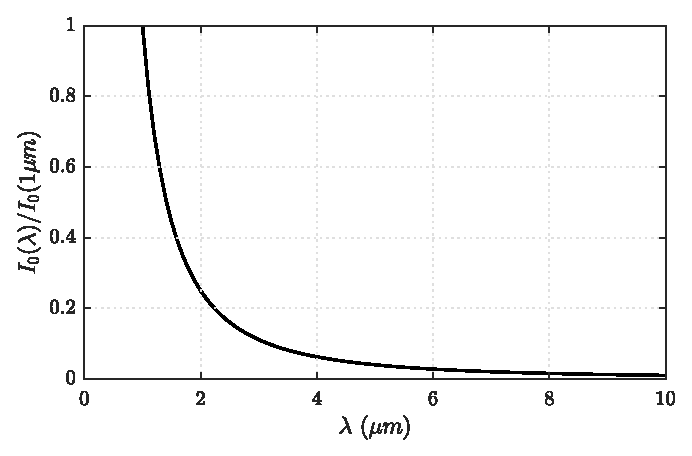
\includegraphics{../matlab/01_introduction/farfield_intensity.eps}
%   \caption{Diffraction-limited far-field intensity of a beam normalized by the performance at 1$\mu$m.}
%   \label{fig:01_farfield_intensity}
% \end{figure}
% As the wavelength of an outgoing beam decreases the diffraction-limited performance greatly improves proportional to $\lambda^{-2}$.
% This provides a strong desire to move towards shorter wavelengths to take advantage of significantly increased diffraction-limited performance.
%
% While diffraction-limited provides the best possible performance, real systems will however have reduced performance.
% The ratio of actual on target intensity, $I(t)$, to diffraction-limited intensity is the Strehl ratio, $\sr$, shown here using the large aperture approximation,
% \begin{equation}
%   \sr(t) = \frac{I(t)}{I_0} \approx \exp\left\{-\left[\frac{2\pi \opdrms(t)}{\lambda}\right]^2\right\}
%   \label{eqn:01_strehl_ratio}
% \end{equation}
% where $\opdrms(t)$ is the spatial root-mean-square of the optical path difference across the aperture.
% The Airborne Laser Laboratory (ALL) which ran from the 1970s to early 1980s used a 10.6 $\mu$m laser and had an estimated Strehl ratio of 95\%\cite{Jumper-2013-8KtN3pue}.
% Figure \ref{fig:01_strehl_ratio} shows a hypothetical case of varying the source wavelength while maintaining the same optical disturbance of ALL.
% \begin{figure}
%   \centering
%   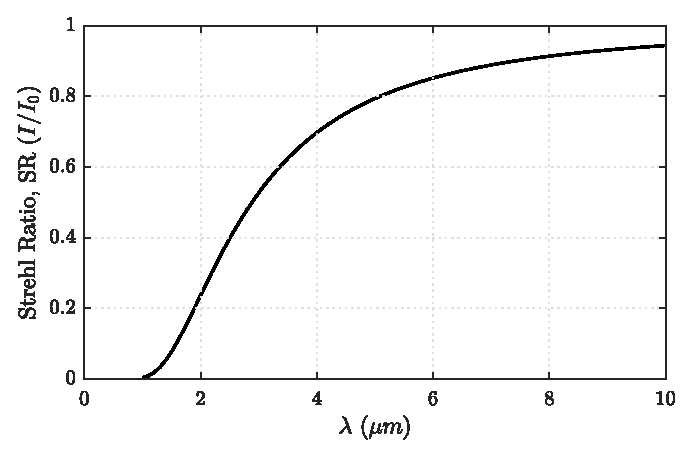
\includegraphics{../matlab/01_introduction/strehl_ratio.eps}
%   \caption{Strehl ratio due to the $\opdrms$ of the Airborne Laser Laboratory at various laser wavelengths.  ALL had an estimated Strehl ratio of 95\% with its 10.6 $\mu$m laser.}
%   \label{fig:01_strehl_ratio}
% \end{figure}
% By changing the laser source to 1 from 10 $\mu$m nets a 100 times increase in diffraction-limited performance, the actual on target intensity drops to practically zero if using a system with the same optical disturbances present on ALL.
%
% As future airborne directed energy systems are developed, their optical disturbances ($\opdrms$) will need to be greatly reduced in order to achieve desired on target performance criteria.
% These systems when tested on the ground in wind tunnels will see optical disturbances that are inherent to the test facility that may be on the order of the optical disturbances of the system its self.
% This research will look at the optical disturbance contamination that comes from the acoustic waves that travel inside of a wind tunnel.
